\subsection{History}
\begin{frame}
  \frametitle{Early Years}
  \begin{itemize}
  \item Began as a start-up in Palo Alto, CA, USA in 2003
  \item Focused from the start on software for mobile devices
  \item Very secretive at the time, even though founders achieved a
    lot in the targeted area before founding it
  \item Finally bought by Google in 2005
  \item Andy Rubin, founder of Android, Inc was also CEO of Danger,
    Inc, a company producing one of the early smartphones, the
    Sidekick
  \end{itemize}
  \begin{center}
    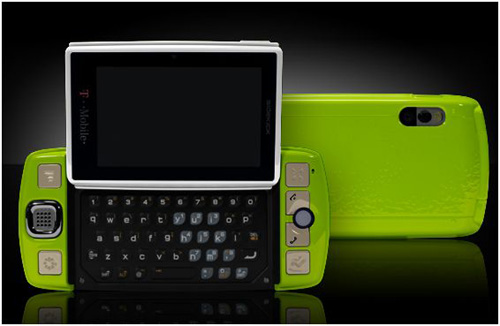
\includegraphics[height=0.4\textheight]{slides/android-introduction-history/sidekick.jpg}
  \end{center}
\end{frame}

\begin{frame}
  \frametitle{Opening Up}
  \begin{itemize}
  \item Google announced the Open Handset Alliance in 2007, a
    consortium of major actors in the mobile area built around Android
    \begin{itemize}
    \item Hardware vendors: Intel, Texas Instruments, Qualcomm,
      Nvidia, etc.
    \item Software companies: Google, eBay, etc.
    \item Hardware manufacturers: Motorola, HTC, Sony Ericsson,
      Samsung, etc.
    \item Mobile operators: T-Mobile, Telefonica, Vodafone, etc.
    \end{itemize}
  \end{itemize}
\end{frame}

\begin{frame}
  \frametitle{Android Open Source Project (AOSP)}
  \begin{itemize}
  \item At every new version, Google releases its source code
    through this project so that community and vendors can
    work with it.
    \begin{itemize}
    \item One major exception: Honeycomb has not been released because
      Google stated that its source code was not clean enough to
      release it.
    \end{itemize}
  \item One can fetch the source code and contribute to it, even though
    the development process is very locked by Google
  \item Only a few devices are supported through AOSP though, only the
    two most recent Android development phones and tablets (part of
    the Nexus brand) and the pandaboard
  \end{itemize}
\end{frame}

\begin{frame}
  \frametitle{Android Releases}
  \begin{itemize}
  \item Each new version is given a dessert name
  \item Released in alphabetical order
  \item Latest releases:
    \begin{itemize}
    \item Android 2.3 Gingerbread
    \item Android 3.X Honeycomb
    \item Android 4.0 Ice Cream Sandwich
    \item Android 4.1/4.2/4.3 Jelly Bean
    \item Android 4.4 KitKat
    \end{itemize}
  \end{itemize}
\end{frame}

\begin{frame}
  \frametitle{Android Versions}
  \begin{center}
    \includegraphics[height=0.8\textheight]{slides/android-introduction-history/history.pdf}
  \end{center}
\end{frame}
